\chapter{Casi d'uso}
I \textbf{casi d'uso} descrivono \textbf{scenari concreti} di \textbf{interazione attori-sistema}, illustrando come il software risponde alle azioni dell'utente per soddisfare un obiettivo specifico.\\
Hanno il ruolo di far comprendere il \textbf{flusso operativo} dell'intero sistema.

\section{Use-Case diagram completo}
L'immagine comprende un \textbf{diagramma Use-Case} dell'intero sistema, comprendente di tutti gli \textit{Attori} del sistema e degli 8 casi d'uso assegnati.
\begin{figure}[h]
	\centering
	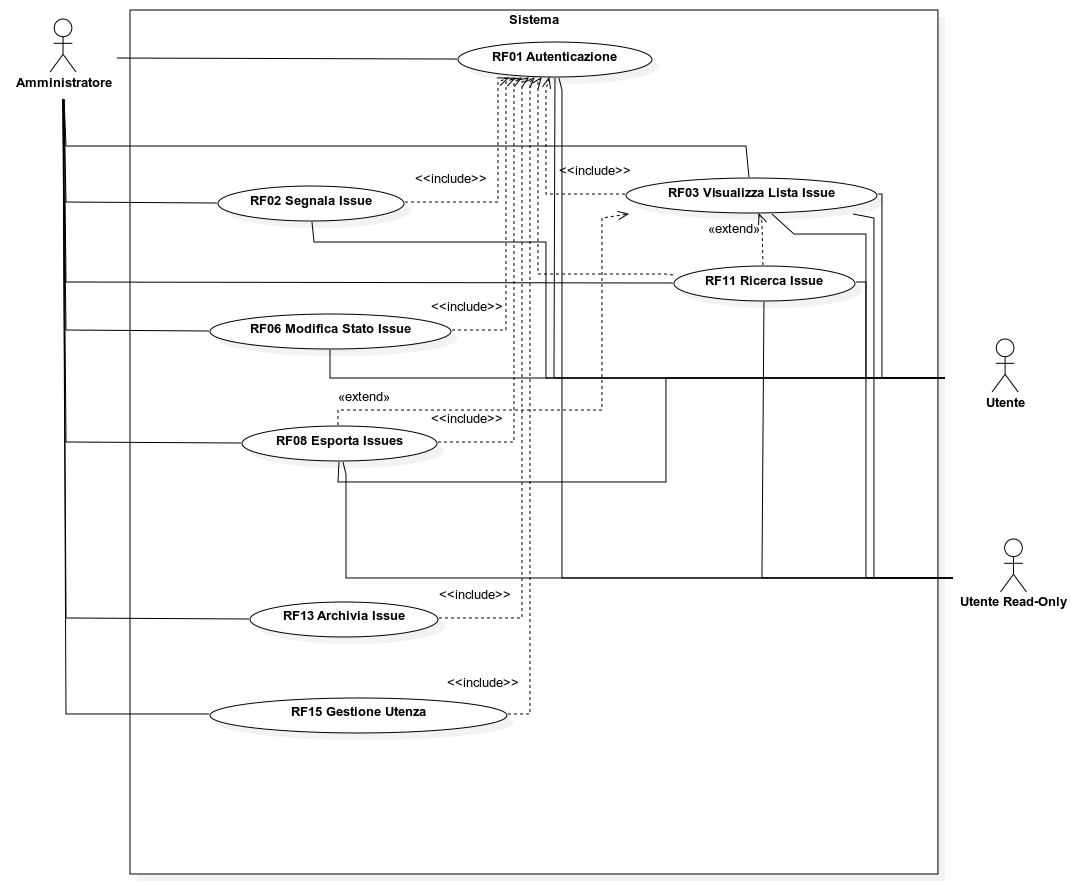
\includegraphics[width=0.7\linewidth]{./Assets/Chapters/use_case.png}
	\caption{Use-Case Completo}
\end{figure}
	
	
\section{Tabella completa Use-Case}
La seguente tabella descrive nel dettaglio i casi d'uso presenti nell'immagine sopra

%---------------------------------------------NON TOCCARE LA TABELLA--------------------------------------------%
\begin{table}[h]
	\caption{Tabella completa Use-Case}
	\begin{tabular}{|c|c|c|c|c|}
		\hline
		ID                           & Titolo                                                                                          & Attori Coinvolti                                                 & Scopo                                                                                                                & Relazioni                                                                                                                                                            \\ \hline
		\rowcolor[HTML]{C8C3BC} 
		UC01                         & \begin{tabular}[c]{@{}c@{}}Autenticazione\\ (RF01)\end{tabular}                                 & \begin{tabular}[c]{@{}c@{}}User\\ Admin\\ Read-only\end{tabular} & \begin{tabular}[c]{@{}c@{}}Accedere al sistema\\ con email e password\end{tabular}                                   & -                                                                                                                                                                    \\ \hline
		UC02                         & \begin{tabular}[c]{@{}c@{}}Segnala Issue\\ (RF02)\end{tabular}                                  & \begin{tabular}[c]{@{}c@{}}User\\ Admin\end{tabular}             & \begin{tabular}[c]{@{}c@{}}Creazione di una nuova\\ issue specificando vari\\ campi\end{tabular}                     & \textless{}\textless{}include\textgreater{}\textgreater RF01                                                                                                         \\ \hline
		\rowcolor[HTML]{C8C3BC} 
		UC03                         & \begin{tabular}[c]{@{}c@{}}Visualizza lista\\ Issue\\ (RF03)\end{tabular}                       & \begin{tabular}[c]{@{}c@{}}User\\ Admin\\ Read-Only\end{tabular} & \begin{tabular}[c]{@{}c@{}}Visualizza l'elenco di \\ issues presenti relative\\ a un progetto specifico\end{tabular} & \textless{}\textless{}include\textgreater{}\textgreater RF01                                                                                                         \\ \hline
		\cellcolor[HTML]{FFFFFF}UC04 & \cellcolor[HTML]{FFFFFF}\begin{tabular}[c]{@{}c@{}}Modifica stato\\ Issue\\ (RF06)\end{tabular} & \begin{tabular}[c]{@{}c@{}}User\\ Admin\end{tabular}             & \begin{tabular}[c]{@{}c@{}}Consente di aggiornare\\ lo stato di una issue,\\ cambiandone i dettagli\end{tabular}     & \textless{}\textless{}include\textgreater{}\textgreater RF01                                                                                                         \\ \hline
		\rowcolor[HTML]{C8C3BC} 
		UC05                         & \begin{tabular}[c]{@{}c@{}}Esporta Issue\\ (RF08)\end{tabular}                                  & \begin{tabular}[c]{@{}c@{}}User\\ Admin\\ Read-Only\end{tabular} & \begin{tabular}[c]{@{}c@{}}Permette di esportare\\ l'elenco di issues in\\ vari formati\end{tabular}                 & \begin{tabular}[c]{@{}c@{}}\textless{}\textless{}include\textgreater{}\textgreater{}RF01\\ \textless{}\textless{}extend\textgreater{}\textgreater{}RF03\end{tabular} \\ \hline
		UC06                         & \begin{tabular}[c]{@{}c@{}}Ricerca Issue\\ (RF11)\end{tabular}                                  & \begin{tabular}[c]{@{}c@{}}User\\ Admin\\ Read-Only\end{tabular} & \begin{tabular}[c]{@{}c@{}}L'utente può cercare una\\ issue utilizzando parole\\ chiave\end{tabular}                 & \begin{tabular}[c]{@{}c@{}}\textless{}\textless{}include\textgreater{}\textgreater{}RF01\\ \textless{}\textless{}extend\textgreater{}\textgreater{}RF03\end{tabular} \\ \hline
		\rowcolor[HTML]{C8C3BC} 
		UC07                         & \begin{tabular}[c]{@{}c@{}}Archivia Issue\\ (RF13)\end{tabular}                                 & Admin                                                            & \begin{tabular}[c]{@{}c@{}}Consente di achiviare le\\ issues, rimuovendola\\ dalla lista principale\end{tabular}     & \textless{}\textless{}include\textgreater{}\textgreater RF01                                                                                                         \\ \hline
		\cellcolor[HTML]{FFFFFF}UC12 & \cellcolor[HTML]{FFFFFF}\begin{tabular}[c]{@{}c@{}}Gestione Utenza\\ (RF15)\end{tabular}        & Admin                                                            & \begin{tabular}[c]{@{}c@{}}Permette di creare,\\ modificare, eliminare\\ altri account\end{tabular}                  & \textless{}\textless{}include\textgreater{}\textgreater RF01                                                                                                         \\ \hline
	\end{tabular}
\end{table}

\clearpage  % <-- AGGIUNGI QUESTO

	\begin{table}
		\centering
		\caption{Cockburn template Use-Case N.02, Segnalazione di una nuova issue}
		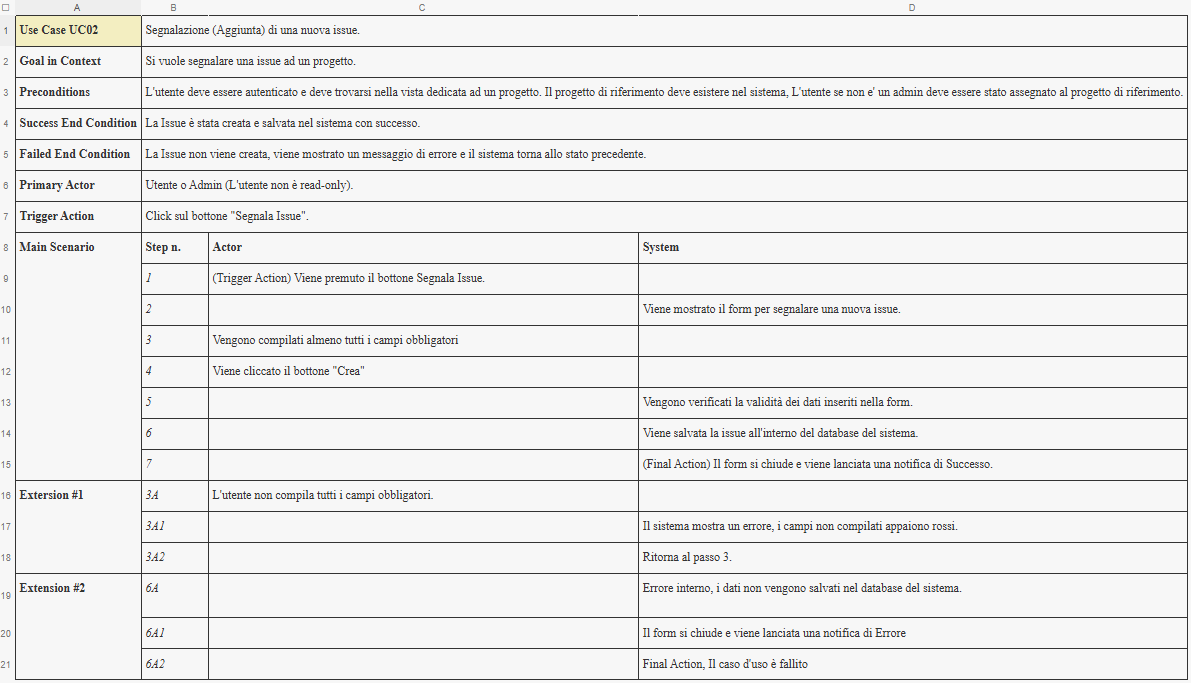
\includegraphics[width=1\linewidth]{./Assets/Chapters/cockburn.png}
	\end{table}

